\documentclass[11pt]{jreport}
\usepackage{wuse_thesis}
\usepackage{indentfirst}
\usepackage{url}	% \url{}コマンド用.URLを表示する際に便利
\usepackage{otf}
\usepackage{xcolor}
\usepackage[dvipdfmx]{graphicx}
%\usepackage{graphicx}  % ←graphicx.styを用いてEPSを取り込む場合有効にする
			% 他のパッケージ・スタイルを使う場合には適宜追加

\newcommand{\RQOne}{Good First Issue に貢献している開発者のうち,新参開発者の割合はどの程度か}
\newcommand{\RQTwo}{熟練者は新参開発者をどの程度待っているか}
\newcommand{\RQThree}{ゲーム理論に基づくと,熟練者はどの程度の期間新参開発者のために GFI の解決を待つのが適切か}
\newcommand{\NIssue}{180,671}
\newcommand{\NTrueIssue}{17,956}
\newcommand{\NGFI}{478}
\newcommand{\NNormal}{17,478}
\newcommand{\NBOT}{5}

\newcommand{\todo}[1]{\colorbox{yellow}{{\bf TODO}:}{\color{red} {\textbf{[#1]}}}}
\newcommand{\change}[1]{\colorbox{green}{{\bf CHANGE}:}{\color{blue} {\textbf{[#1]}}}}
\newcommand{\new}[1]{\colorbox{cyan}{{\bf NEW}:}{\color{black} {\textbf{[#1]}}}}

%%%%%%%%%%%%%%%%%%%%%%%%%%%%%%%%%%%%%%%%%%%%%%%%%%%%%%%%%%%%%%%%%%%%%%%%

%%
%% 主に表紙を作成するための情報
%%

%%  タイトル(修論の場合は英語表記も指定)
\title{新参開発者向けの障害対応のジレンマ〜熟練者が介入するタイミングの分析〜}
%\etitle{Test\\Test\\Test}

%%  著者名(修論の場合は英語表記も指定)
\author{中井 大雄}
%\eauthor{Akinori Ihara}

%% 卒業論文・修士論文(以下のどちらかを選択)
\bachelar	% 卒業論文(4年生用)
%\master  	% 修士論文(M2用)

%%  学科・クラスタ
\department{システム工}
%\department{デザイン情報}
%\department{デザイン科学}

%%  学生番号
\studentid{60246191}

%%  卒業年度
\gyear{2024}		% 提出年が2022年なら,2021年度

%%  論文提出日
\date{2025年2月12日}	% 修士の場合は月(2021年2月)までとし,英語表記も指定
%\edate{February 2021}	% 修士の場合,こちら(英語表記)も有効化

%%%%%%%%%%%%%%%%%%%%%%%%%%%%%%%%%%%%%%%%%%%%%%%%%%%%%%%%%%%%%%%%%%%%%%%%

\begin{document}

\maketitle

%%
%%  概要
%%
\begin{abstract}
本研究では,オープンソースソフトウェア(OSS)開発において,新参開発者の課題解決を熟練者がどれだけ待っているかを実証データとゲーム理論での分析を比較する.

OSSプロジェクトの持続可能な開発には新参開発者を獲得する必要がある.新参参入の障壁を減らすために,一部のOSSプロジェクトでは新参開発者が取り組みやすい課題に対して「Good First Issue(GFI)」と呼ばれるラベルを付与している.新参開発者が初めに取り組むべき課題を明示することで,プロジェクトに精通していない開発者でも新たに開発に参加しやすい環境を作っている.ところが,先行研究では新参開発者ではない熟練の開発者がGFIを解決している事例が多くみられるとの指摘があった.

本研究では,GFIを解決している開発者の経験値を調査し,GFIが本来の目的通り新参開発者に解決されているかを分析する.また,調査ではGFIに興味を示す新参開発者が長期間現れなかった場合に,熟練者が代わってGFIを解決するケースが見られた.熟練者はどの程度の期間GFIを代行して解決するのを待っているかを調べる.

収集した\NIssue 件のIssueをGFIと通常Issueに分類し,解決した開発者の経験値を比較する(RQ1).また,Issueが開放されている時間とIssueを解決した開発者の経験値との関係を分析する(RQ2).以上の結果を踏まえて,ゲーム理論で提案される待機時間と実証データを比較し,考察する(RQ3).

\todo{考察と結論の概要}
\end{abstract}

%%  目次
\tableofcontents

%%  図目次 (図目次をいれたければ以下のコメントをはずす)
%\listoffigures

%%  表目次 (表目次をいれたければ以下のコメントをはずす)
%\listoftables

\newpage
\pagenumbering{arabic}	% 以降のページ番号を算用数字に

%%%%%%%%%%%%%%%%%%%%%%%%%%%%%%%%%%%%%%%%%%%%%%%%%%%%%%%%%%%%%%%%%%%%%%%%

%%
%%  本文はここから
%%

\chapter{はじめに}

OSSプロジェクトの多くはボランティアの開発者によって支えられている\cite{definding}.ボランティア開発者は任意のタイミングでプロジェクトへの参加・離脱の意思を自由に決定できるため,安定的に開発に携わる人員を確保することは困難である.これを踏まえ,持続可能なOSS開発のためにOSSプロジェクトは常に新参の貢献者(以下,新参開発者)を募ることで,十分な人員を確保し安定的な開発体制を維持することが重要である.新参開発者の参入障壁を下げるために,メンタリング制度\cite{menter1}\cite{menter2}や新参開発者向けのポータルサイト\cite{portal}を用意するなど,様々な方法でオンボーディング支援を行っている.
\todo{継続の話がノイズになっている}

新参開発者が新しいOSSプロジェクトに貢献するにあたってIssueの内容を正確に理解することは困難であるため,タスクに関する情報を提供することやコミュニティから具体的な指示を促す必要性が指摘されている\cite{choice}.一部のプロジェクトでは,新参開発者がプロジェクトで最初の貢献として選ぶのに適したIssueに対して「Good First Issue\footnote{https://docs.github.com/en/issues/using-labels-and-milestones-to-track-work/managing-labels}(GFI)」というラベルを付与している.このラベルによって,新参開発者は自身が貢献すべきIssueを簡単に見つけることができるため,OSSプロジェクトへの参加障壁を下げることができる.
しかしながら,GFIに着目した先行研究\cite{GFI}によると,新参開発者ではない経験豊富な開発者がGFIに貢献を行っているとの指摘がある.熟練者によってGFIが解決される理由として,先行研究では新参開発者に適さないIssueに対してGFIラベルを付与していたことが原因であると考えられている.このほかの理由として,長期間にわたって新参開発者が現れずにGFIの解決が放置された場合について私は着目した.本来,新参開発者のために置いておくべきGFIを熟練者が先に解決してしまうことは,新参開発者の参入を遠ざけることになり,OSSプロジェクトの持続可能性にとっては問題となる.介入のタイミングが遅すぎる場合はプロジェクトに悪影響があり,介入のタイミングが早すぎる場合は新参開発者の参入を阻害してしまうというジレンマを熟練者は抱えている.

本研究の目的は,熟練者がサポートする適切なタイミングを明らかにすることである.つづく2章では,関連研究の紹介と本研究の位置づけを行い,3つのResarch Question(RQ)を立てる.
\vskip\baselineskip
\noindent\textbf {RQ1: \RQOne }\\

Issueを解決した開発者の経験値を分析する.GFIと通常Issueを比較することで,GFIは目的通り新参開発者に解決されているかを明らかにする.
\vskip\baselineskip
\noindent\textbf {RQ2: \RQTwo }\\

Issueが開放されている時間とIssueを解決した開発者の経験値との関係を分析する.GFIと通常Issueを比較することで,熟練者は新参開発者のためにGFIの解決を待っているかを明らかにする
\vskip\baselineskip
\noindent\textbf {RQ3: \RQThree }\\
\todo{RQ3要約}

\todo{RQ要約}
\vskip\baselineskip
3章では,分析方法の説明とその結果を説明する.4章では,3章の結果を分析し,ゲーム理論による分析と実際の熟練者のふるまいはどのように異なるか・違いが生じる理由について考察する.6章では,本研究の結論を述べる.

\chapter{背景}\label{chap:fig-tab-exp}

\section{OSSプロジェクトによる新参開発者獲得の取り組みと課題}

\subsection{OSSプロジェクトにとっての新参開発者獲得の重要性}

%OSSプロジェクトの持続可能性のためには新参開発者が必要である 

オープンソースソフトウェア(OSS: Open Source Software)は,インターネットを通じてソースコードが公開され,誰でも自由に使用・改変・再配布できるソフトウェアのことを指す.
私たちが普段利用するアプリケーション(GIMP, OpenOffice)やプログラミング言語(Perl, Python)などはOSSとして開発が行われている.OSSの開発者の多くは金銭などの報酬を得ているのではなく,ボランティアとしてプロジェクトに貢献している\cite{definding}.ボランティア開発者はプロジェクトへの参加が自由であることと同時に,プロジェクトからの離脱も自由にできる.そのため,ボランティア開発者の動機を理解し,流動性を把握することは,OSSプロジェクトの持続可能な開発・保守のために重要である.
安定的に開発者を確保するためには,既存の開発者に長期的な貢献を促すほかに,新参開発者を獲得することも重要である.先行研究\cite{OTC}では,一度だけ貢献を行ったがすぐにプロジェクトから離脱する開発者(One Time Contributors)の貢献動機を分析し,オンボーディング支援の方法が研究されている.

\subsection{新参参入者にとってのOSSプロジェクトの参入障壁}
新参開発者にとって,技術的・社会的な要因がプロジェクトへの参入障壁となっていることが指摘されている\cite{sosial}.特に,新参開発者が初めての投稿を行う場合は既存の開発者とのコミュニケーションなど社会的な要因が障壁となる\cite{social barries}.そこで,新参開発者とのコミュニケーションを支援する目的でメンタリング制度\cite{menter1}\cite{menter2}を導入するプロジェクトもある.新参開発者と密にコミュニケーションを取り,共同で課題に取り組んだり,新参開発者が実装したソースコードへ積極的にフィードバックを行うメンターを設けることで,オンボーディングの支援を行う.しかし,これらの方法はメンターへの負担が大きいため,多くのプロジェクトは導入することが容易でない.プロジェクトにとって負担にならない方法でオンボーディング支援を行う方法が求められている.

\subsection{新参開発者の参入を促すためのissueのラベリング}
OSS開発の主要なプラットフォームの1つであるGitHubでは,バグ報告や機能追加の要求などのプロジェクトが取り組むべき課題をIssue\footnote{https://docs.github.com/en/issues/tracking-your-work-with-issues/about-issues}という単位で管理している.GitHub上でのIssueの表示画面を図\todo{図番号}に示す.本文では投稿者がIssueの内容を説明し,具体的な報告や要望が記載される.これを受けて,開発者はIssue Commentという形で投稿者や他の開発者と議論を交わしながら課題の解決をする.ソースコードの変更が必要な場合,開発者はPull Request\footnote{https://docs.github.com/en/issues/tracking-your-work-with-issues/about-issues}(以下,PR)という機能を用いて作成したコードのレビューを依頼する.Pull Requestはソースコードなどの変更をリポジトリに提案する機能である.レビューを通してバグなどが解消され,問題がないと判断されたコードはリポジトリに取り込まれる.Issueの状態はstateと呼ばれる機能で管理されており,課題が解決されたIssueはstateがOPEN状態からCLOSED状態となり,議論が終了する.

%-------------------
\begin{figure*}[t]
\centerline{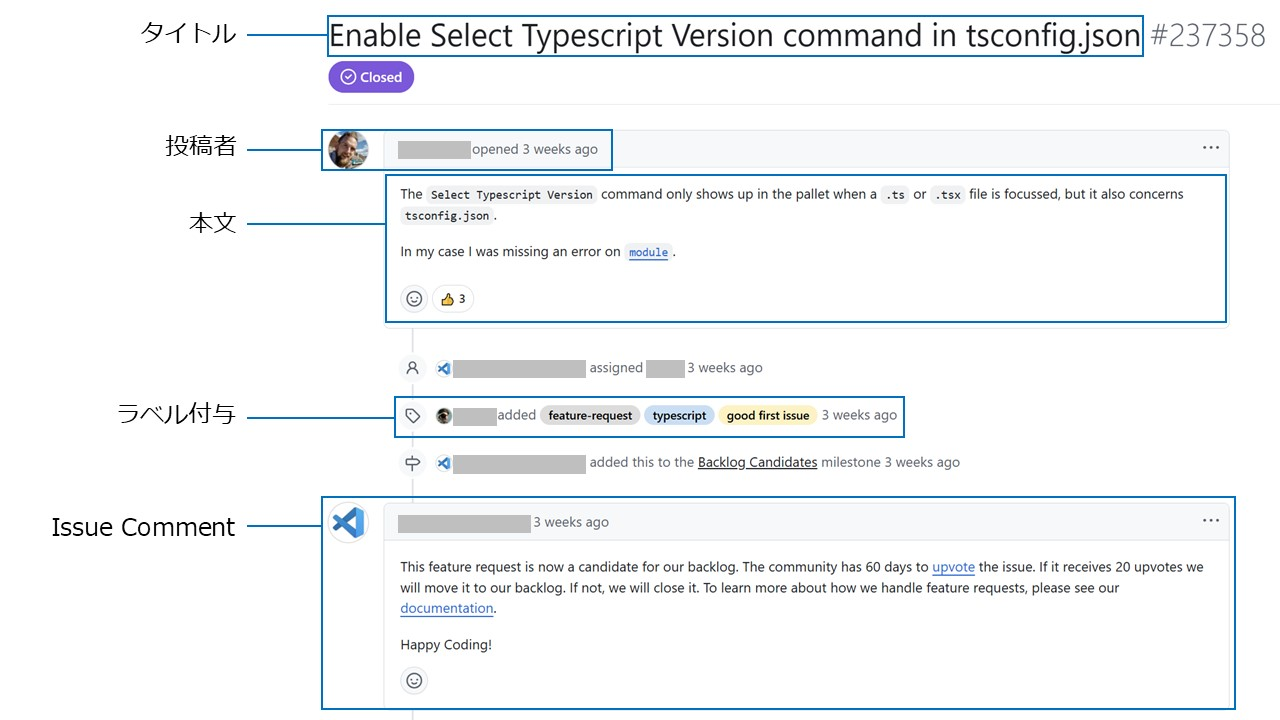
\includegraphics[width=0.9\linewidth]{@BSthesis2024_Nakai/BSthesis2024_Nakai_fig/issue_page.jpg}}
\caption{GitHubのIssueの画面}
\label{fig:milestone}
\end{figure*}
%-------------------

GitHubではラベル(label\footnote{https://docs.github.com/en/issues/using-labels-and-milestones-to-track-work/managing-labels})という機能を用いて,IssueやPRを分類して管理することができる.例えば,バグ報告のIssueに対しては``bug"というラベルが,機能要求に対しては``enhancement"といったラベルが付与されることが多い.このようにIssueの特徴をラベル付けしておくことで,膨大なIssueから目的のラベルでフィルタリングして検索することで探したい種類のIssueを容易に見つけることができる.多くの場合,ラベリングはメンテナと呼ばれるプロジェクトの中心的な管理者がIssueの内容を確認し,適したラベルを付与する.
一部のOSSプロジェクトでは,新参開発者にとって解決が容易なIssueに対して``good first issue"や``easy to fix"などのラベルを付与して分類している.このようなIssueは``Good First Issue(GFI)”と呼ばれ,新参開発者の新規参入の障壁を軽減する目的で使用されている.

\subsection{Good First Issueが熟練者によって解決されている問題}
新参開発者の新規参入を容易にする目的でGFIは使用されるが,GFIに着目した先行研究\cite{GFI_half}によると,GFIのうち半数近くは熟練者によって解決されているとの指摘があった.また,熟練者によってGFIが解決される理由として新参開発者に適さないIssueに対してGFIラベルを付与していたことや,Issueの説明内容が新参開発者にとって説明不足だったことが原因であると考えられている.このように,GFIは本来の目的である新参開発者の獲得に十分に寄与できていないという課題を抱えている.

\section{ゲーム理論に基づくOSS開発者の行動分析 }

\subsection{ゲーム理論関連の用語 }

ゲーム理論とは様々な意思決定の相互依存関係を数学的で厳密な方法論を用いて分析する学問である.経済学だけでなく社会学や工学など幅広い分野でプレイヤーの戦略分析に応用されている.
ここでは,本論文で用いるゲーム用語に関する用語について参考文献\cite{game_theory}に沿って定義する.

\begin{description}
\item[戦略型ゲーム] 戦略型ゲームは,ゲームに参加するプレイヤー,プレイヤーが選択する戦略,戦略の結果プレイヤーが得る効用値から構成される.プレイヤーは同時に戦略を選び,その結果プレイヤーの効用値が決まる.
\item[非協力ゲーム] プレイヤー同士が合意せずに戦略を選択する場合,プレイヤーは相手プレイヤーの戦略を予測したうえで,自らの戦略を選択しなければならない.このように,プレイヤーが互いの戦略を独立に決定するような状況を非協力ゲームという.
\item[混合戦略]各プレイヤーが確率分布に基づいて自身の戦略を決定する場合,この戦略を混合戦略という.
\item[期待効用値]各プレイヤーが混合戦略を用いるとき,期待される効用値は戦略を選択する確率と戦略で得られる効用値を掛け合わせた確率分布で表現できる.この確率分布を期待効用値という. 
\item[ナッシュ均衡]混合戦略において,プレイヤーが戦略を変更することによって自身の得ることができる期待効用値を最大化できない場合,この選択の組をナッシュ均衡(Nash Equilibrium, NE)と呼ぶ. NEは両プレイヤーが最適な戦略を選択した場合に現れる非協力ゲームの解の一種である.
\item[] 
\end{description}


実際のOSS開発においては新参開発者,熟練者ともに複数人いることが想定されるが,本論文では問題を単純化するためにプレイヤーAを新参開発者,プレイヤーBを熟練者とするような,2プレイヤーのゲームと仮定する.
Issueがあったとき,開発者は貢献する,貢献しないという2種類の戦略を選択することになる.
また,熟練者が貢献する確率をp,新参開発者が貢献する確率をqとするような確率変数に基づく混合戦略を想定する.

\subsection{スノードリフトゲームの概要 }
ゲーム理論を用いた分析として,2人のプレイヤーが共通の利益のために協力するかどうかを選択するスノードリフトゲームを例に挙げて説明する.2人のプレイヤーAとBは道路が雪で埋まり通行できない状況に直面している.各プレイヤーは雪かきをする(Cooperate, C)もしくは待機する(Defect, D)のいずれかの戦略を選択できる.道路が通行できた場合,両プレイヤーは利得bを得られる.1人で雪かきをした場合体力を消耗するため,コスト$c_1$がかかる.2人で協力して雪かきをした場合,消耗する体力は少なく済むため,コスト$c_2$($c_2 < c_1$)がかかるとする.

この場合,各プレイヤーが得る効用は表2.2\todo{番号}のようになる.
両プレイヤーが雪かきする場合,両プレイヤーは共通して$b - c_2$の効用値を得る.片方のプレイヤーが雪かきをし,もう片方のプレイヤーがしない場合,雪かきをしたプレイヤーは$b - c_1$,雪かきをしなかったプレイヤーは$b$の効用値を得る.両方のプレイヤーが雪かきをしない場合,両プレイヤーは共通して$0$の効用値を得る.
ここで,両プレイヤーは自身の効用が最大になる最適戦略を選ぶとする.プレイヤーAは雪かきをしなかった場合に得られる$b$の効用値が期待できる最大の効用値であるため,雪かきをしない.同様の理由でプレイヤーBも雪かきをしない.この時両者が得る効用値は$(0, 0)$となり,どちらも効用を得られない最悪の状態になる.プレイヤーは協力しなければ最大の効用が得られるが,両者が同じ戦略の場合には効用が最小となるジレンマを抱えている.スノードリフトゲームは協力と自己利益のバランスを扱うため,OSS開発の分析に適切なモデルである.
%-------------------
\begin{figure*}[t]
\centerline{
\includegraphics[width=0.9\linewidth]{@BSthesis2024_Nakai/BSthesis2024_Nakai_fig/snowdrift.png}}
\caption{スノードリフトゲームの戦略と効用}
\label{fig:milestone}
\end{figure*}
%-------------------

\section{動機・リサーチクエスチョン(RQ)}

2.1.4節で述べた通り,GFIの半数は熟練者によって解決されており,本来の目的である新参開発者の獲得に十分に寄与できていないという課題を抱えている.先行研究\cite{GFI}\cite{GFI_half}では不適切なラベリングやIssue内容の説明不足が原因だと分析している.このほかの理由として,長期間にわたって新参開発者が現れずにGFIの解決が放置された場合に熟練者が代わってGFIを解決するケースに私は着目した.

本来,新参開発者のために置いておくべきGFIを熟練者が先に解決してしまうことは,新参開発者の参入を遠ざけることになり,OSSプロジェクトの持続可能性にとっては問題となる.逆に介入のタイミングが遅すぎる場合は未解決のIssueを放置しているメンテナンス不足なプロジェクトであるとユーザに不信感を与えることとなる.介入のタイミングが早すぎても遅すぎてもプロジェクトの成長に悪影響を及ぼすというジレンマを熟練者は抱えている.
そこで,本論文では以下の3つのRQを設定し,GFIへの介入のタイミングについて分析する.

\vskip\baselineskip
\noindent\textbf {RQ1: \RQOne }\\

Issueを解決した開発者の経験値を分析する.GFIと通常Issueを比較することで,GFIは目的通り新参開発者に解決されているかを明らかにする.
\vskip\baselineskip
\noindent\textbf {RQ2: \RQTwo }\\

Issueが開放されている時間とIssueを解決した開発者の経験値との関係を分析する.GFIと通常Issueを比較することで,熟練者は新参開発者のためにGFIの解決を待っているかを明らかにする
\vskip\baselineskip
\noindent\textbf {RQ3: \RQThree }\\
\todo{RQ3要約}

\chapter{ケーススタディ}

\section{データセット}
\subsection{対象リポジトリ}
GitHub上でGood First Issueを運用しており十分なデータが得られるプロジェクトとして,今回はmicrosoftのVSCodeプロジェクトを対象とした.また,現在進行中のIssueを除外するため,CLOSED状態になっているIssueのみを分析の対象とした.データ収集期間はvscodeプロジェクトが作成された2015年9月3日から2025年1月28日までとした.

以上の条件に合うIssue \NIssue 件のうち,プルリクエストが存在しないなどの理由でIssueを解決した開発者が分からないものを除外したものが\NTrueIssue 件であった.これらのラベル情報を参照し,``Good First Issue"ラベルがついているものをGFI,ついていないものを通常Issueとする.その結果,GFIは \NGFI 件,通常Issueは \NNormal 件であった.

\subsection{ボットアカウントの除外}
Issueに関係する開発者としてボットアカウントが取得される場合がある.これらのアカウントは今回分析の対象とする新参開発者・熟練者どちらでもないためデータセットから除外する.多くのボットアカウントはユーザ名に``user[bot]"のようにボットであることを示す表記をしている.取得した開発者から目視でボットアカウントであると確認できた開発者をボットリストとしてリストアップし,\NBOT 件のユーザを除外した.

\subsection{経験値の定義}
Issueに紐づけられているプルリクエスト(PR)のうち,最終的にmainブランチにマージされたものを作成した開発者をIssueの解決者とする.
解決者が新参開発者か熟練者かを2値で分類することは困難なため,開発者の経験値を連続値で取得する.経験値の定義はPR作成時点での当該リポジトリにおける過去のPR作成数とIssueに対するコメントの作成数を合わせたものとする.経験値の定義にIssue Commentを入れたのはPRの作成まで行かずとも,Issueに対して何らかの行動を起こすことでも十分に新参開発者にとって重要な参加経験であると考えたからである.また,参照する経験値は対象IssueがCLOSED状態になった時点のものとする.本来であれば,対象Issueが解決された時点であるPR作成時点の経験値を取得すべきだが,APIを利用したデータ取得の都合でPRの作成時刻を確実に取得できない場合があるため,CLOSED状態になった時刻を利用する.

%-------------------
\begin{figure*}[t]
\centerline{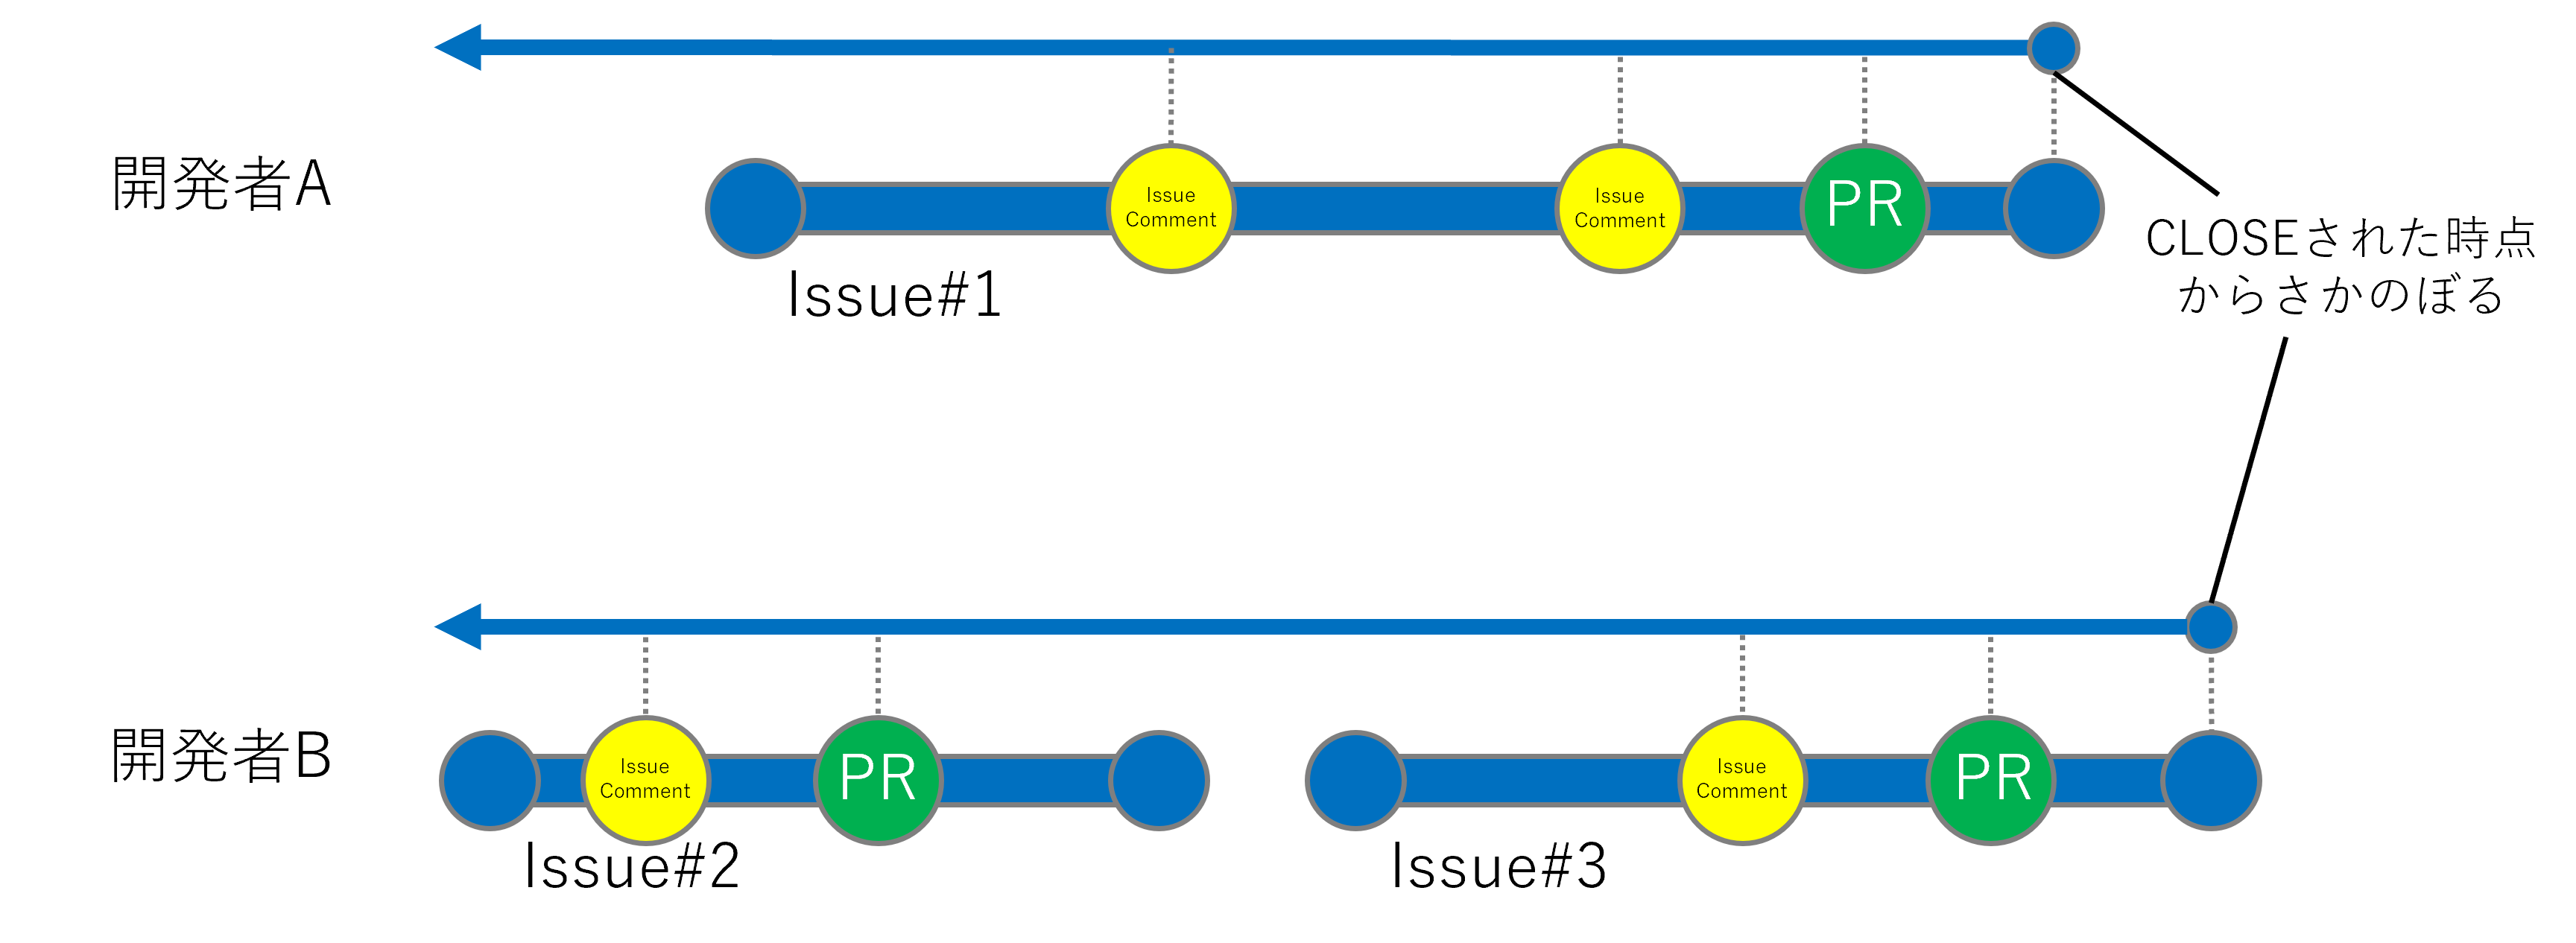
\includegraphics[width=0.9\linewidth]{@BSthesis2024_Nakai/BSthesis2024_Nakai_fig/exp.png}}
\caption{経験値の算出方法}
\label{fig:milestone}
\end{figure*}
%-------------------

経験値の算出方法について,図\todo{番号}を例に説明する.今,開発者AはIssue#1を解決した.Issue\#1がCLOSEされるより以前に,開発者AはIssue\#1にて2件のIssue Commentと1件のPRを作成している.よって,開発者Aの経験値はこれらを合わせた3となる.開発者BはIssue\#3を解決した.Issue\#3が解決されるより以前に,開発者BはIssue\#2にて1件のIssue Commentと1件のPRを,Issue\#3にて1件のIssue Commentと1件のPRを作成している.よって,開発者Bの経験値はこれらを合わせた4となる.

\section{RQ1: \RQOne}

\subsection{概要}

先行研究\cite{GFI}にあったGFIを熟練の開発者が解決しているという指摘が正しいかを分析する.熟練者がIssueを解決しているのはどの程度の割合なのか,GFIとそうでないIssueの割合を比較する.GFIが新参開発者向けのIssueであるならば,通常Issueに比べて熟練者の割合が少なくなるはずである.実証データを分析し,GFIが本来の役割を果たしているかを検証する.

\subsection{手法}
3.1節で説明した\NIssue 件のIssueから,解決した開発者の経験値を取得する.
リポジトリのすべてのIssueについて解決者の経験値を取得し,GFIと通常Issueでは貢献した開発者の経験値分布にどのような違いがみられるかを箱ひげ図で比較する.また,2つの分布に有意な差がみられるかをマンホイットニーのU検定を用いて分析する.p値が0.05以下の場合に有意差ありと判断する.また,GFIと通常Issueでデータの数が大きく異なるため,効果量についても分析する.

\subsection{結果}

結果を図3.1\todo{番号確認}に示す.縦軸はIssueを解決した人の経験値で,対数軸で表現した.GFIと通常Issueに有意差はないと帰無仮説を立てたとき,マンホイットニーのU検定を行うとp値は0.00000であった.また,効果量は-0.668であった.このことから,2つの分布に有意な差があるといえる.

%-------------------
\begin{figure*}[t]
\centerline{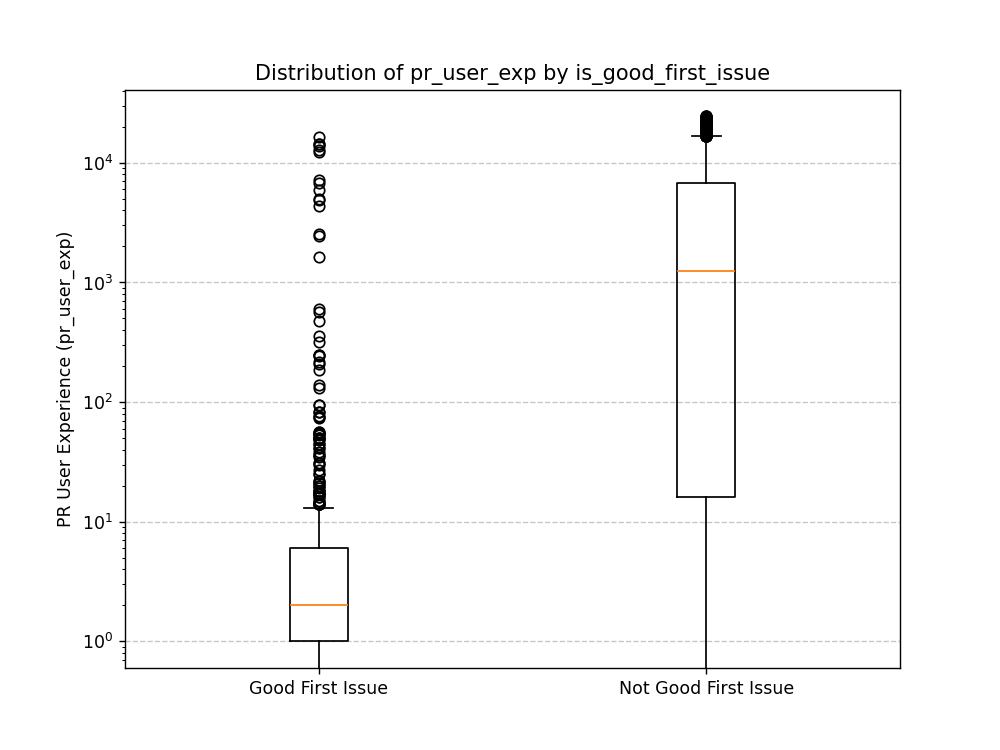
\includegraphics[width=0.9\linewidth]{@BSthesis2024_Nakai/BSthesis2024_Nakai_fig/2025-02-03_11h12_00.png}}
\caption{経験値の箱ひげ図}
\label{fig:milestone}
\end{figure*}
%-------------------


\section{RQ2: \RQTwo}

\subsection{概要}

通常Isuueはすべての開発者が任意のタイミングで取り組むことができるため,Issueが作られてからPRの作成を申し出るまでが早かった開発者が解決する.一方GFIは新参開発者によって解決されることが望ましいため,熟練者は解決できそうな内容であっても取り組みを見送る.ただし,未解決のIssueを放置しておくことはメンテナンスが十分になされていないとユーザに判断されプロジェクトに対する信頼性が低下する.このことはプロジェクトにとって望ましくないため,長期間,新参開発者からの解決の申し出がなかったGFIは熟練者が解決する.そこで,熟練者は新参開発者が現れるのをどの程度の期間待っているのかに注目する.Issueができてから解決されるまでの期間をGFIと通常Issueで比較する.通常IssueよりもGFIのほうが解決までに時間がかかっていれば,熟練者は新参開発者のためにGFIの解決を待っているといえる.

\subsection{手法}
3.1節で説明したリポジトリの \NIssue 件のIssueを用いる.開発者の経験値は3.2.2節と同じものを使う.
Issueが新参開発者のために開放されている時間を取得する.開放期間の定義はIssueが作られた時間から,CLOSED状態になった時間までとする.

リポジトリのすべてのIssueについて開放期間を取得し,GFIと通常Issueでは解決までの期間にどのような違いがみられるかを箱ひげ図で比較する.また,2つの分布に有意な差がみられるかをマンホイットニーのU検定を用いて分析する.p値が0.05以下の場合に有意差ありと判断する.また,GFIと通常Issueでデータの数が大きく異なるため,効果量についても分析する.
さらに,開放期間と解決者の経験値の関係についても分析する.Issueの開放期間とIssueを解決した開発者の経験値の関係を散布図で表現し,GFIと通常Issueでどのような違いがみられるかを分析する.

\subsection{結果}
箱ひげ図の結果を図\todo{番号}に示す.縦軸はIssueを解決した人の経験値で,対数軸で表現した.GFIと通常Issueに有意差はないと帰無仮説を立てたとき,マンホイットニーのU検定を行うとp値は0.00000であった.また,効果量は0.337であった.このことから,2つの分布に有意な差があるといえる.

%-------------------
\begin{figure*}[t]
\centerline{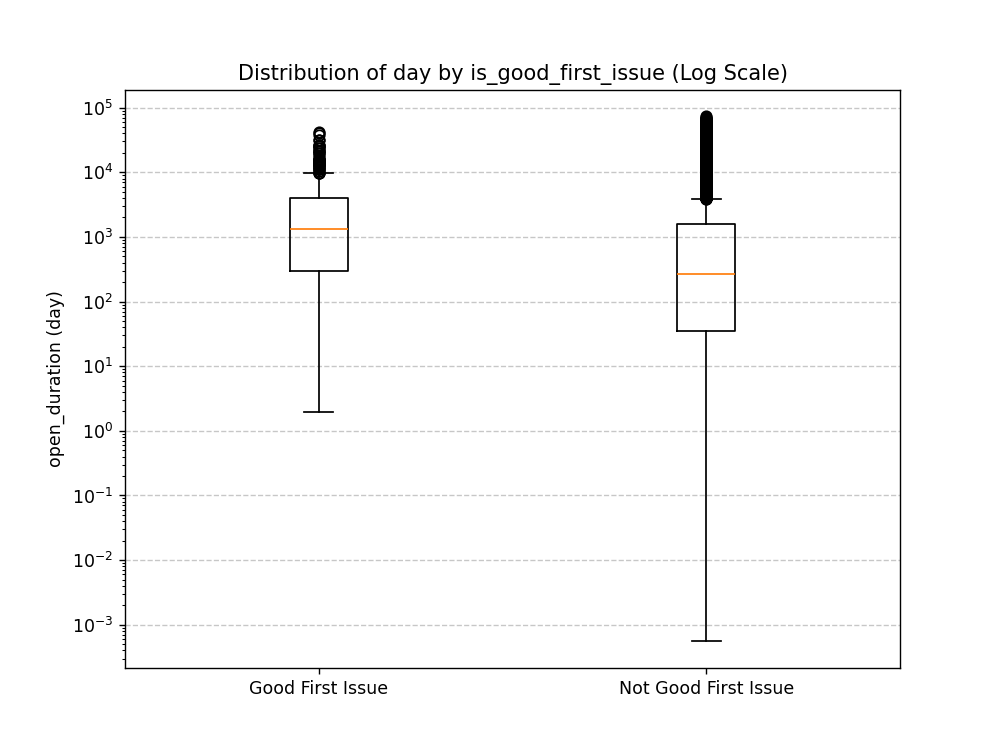
\includegraphics[width=0.9\linewidth]{@BSthesis2024_Nakai/BSthesis2024_Nakai_fig/time_box.png}}
\caption{開放期間の箱ひげ図}
\label{fig:milestone}
\end{figure*}
%-------------------

散布図の結果を図\todo{番号}に示す.横軸はIssueが開放されている期間,縦軸はIssueを解決した人の経験値でそれぞれ対数軸で表現した.破線は縦軸・横軸の中央値を表現している.

%-------------------
\begin{figure*}[t]
\centerline{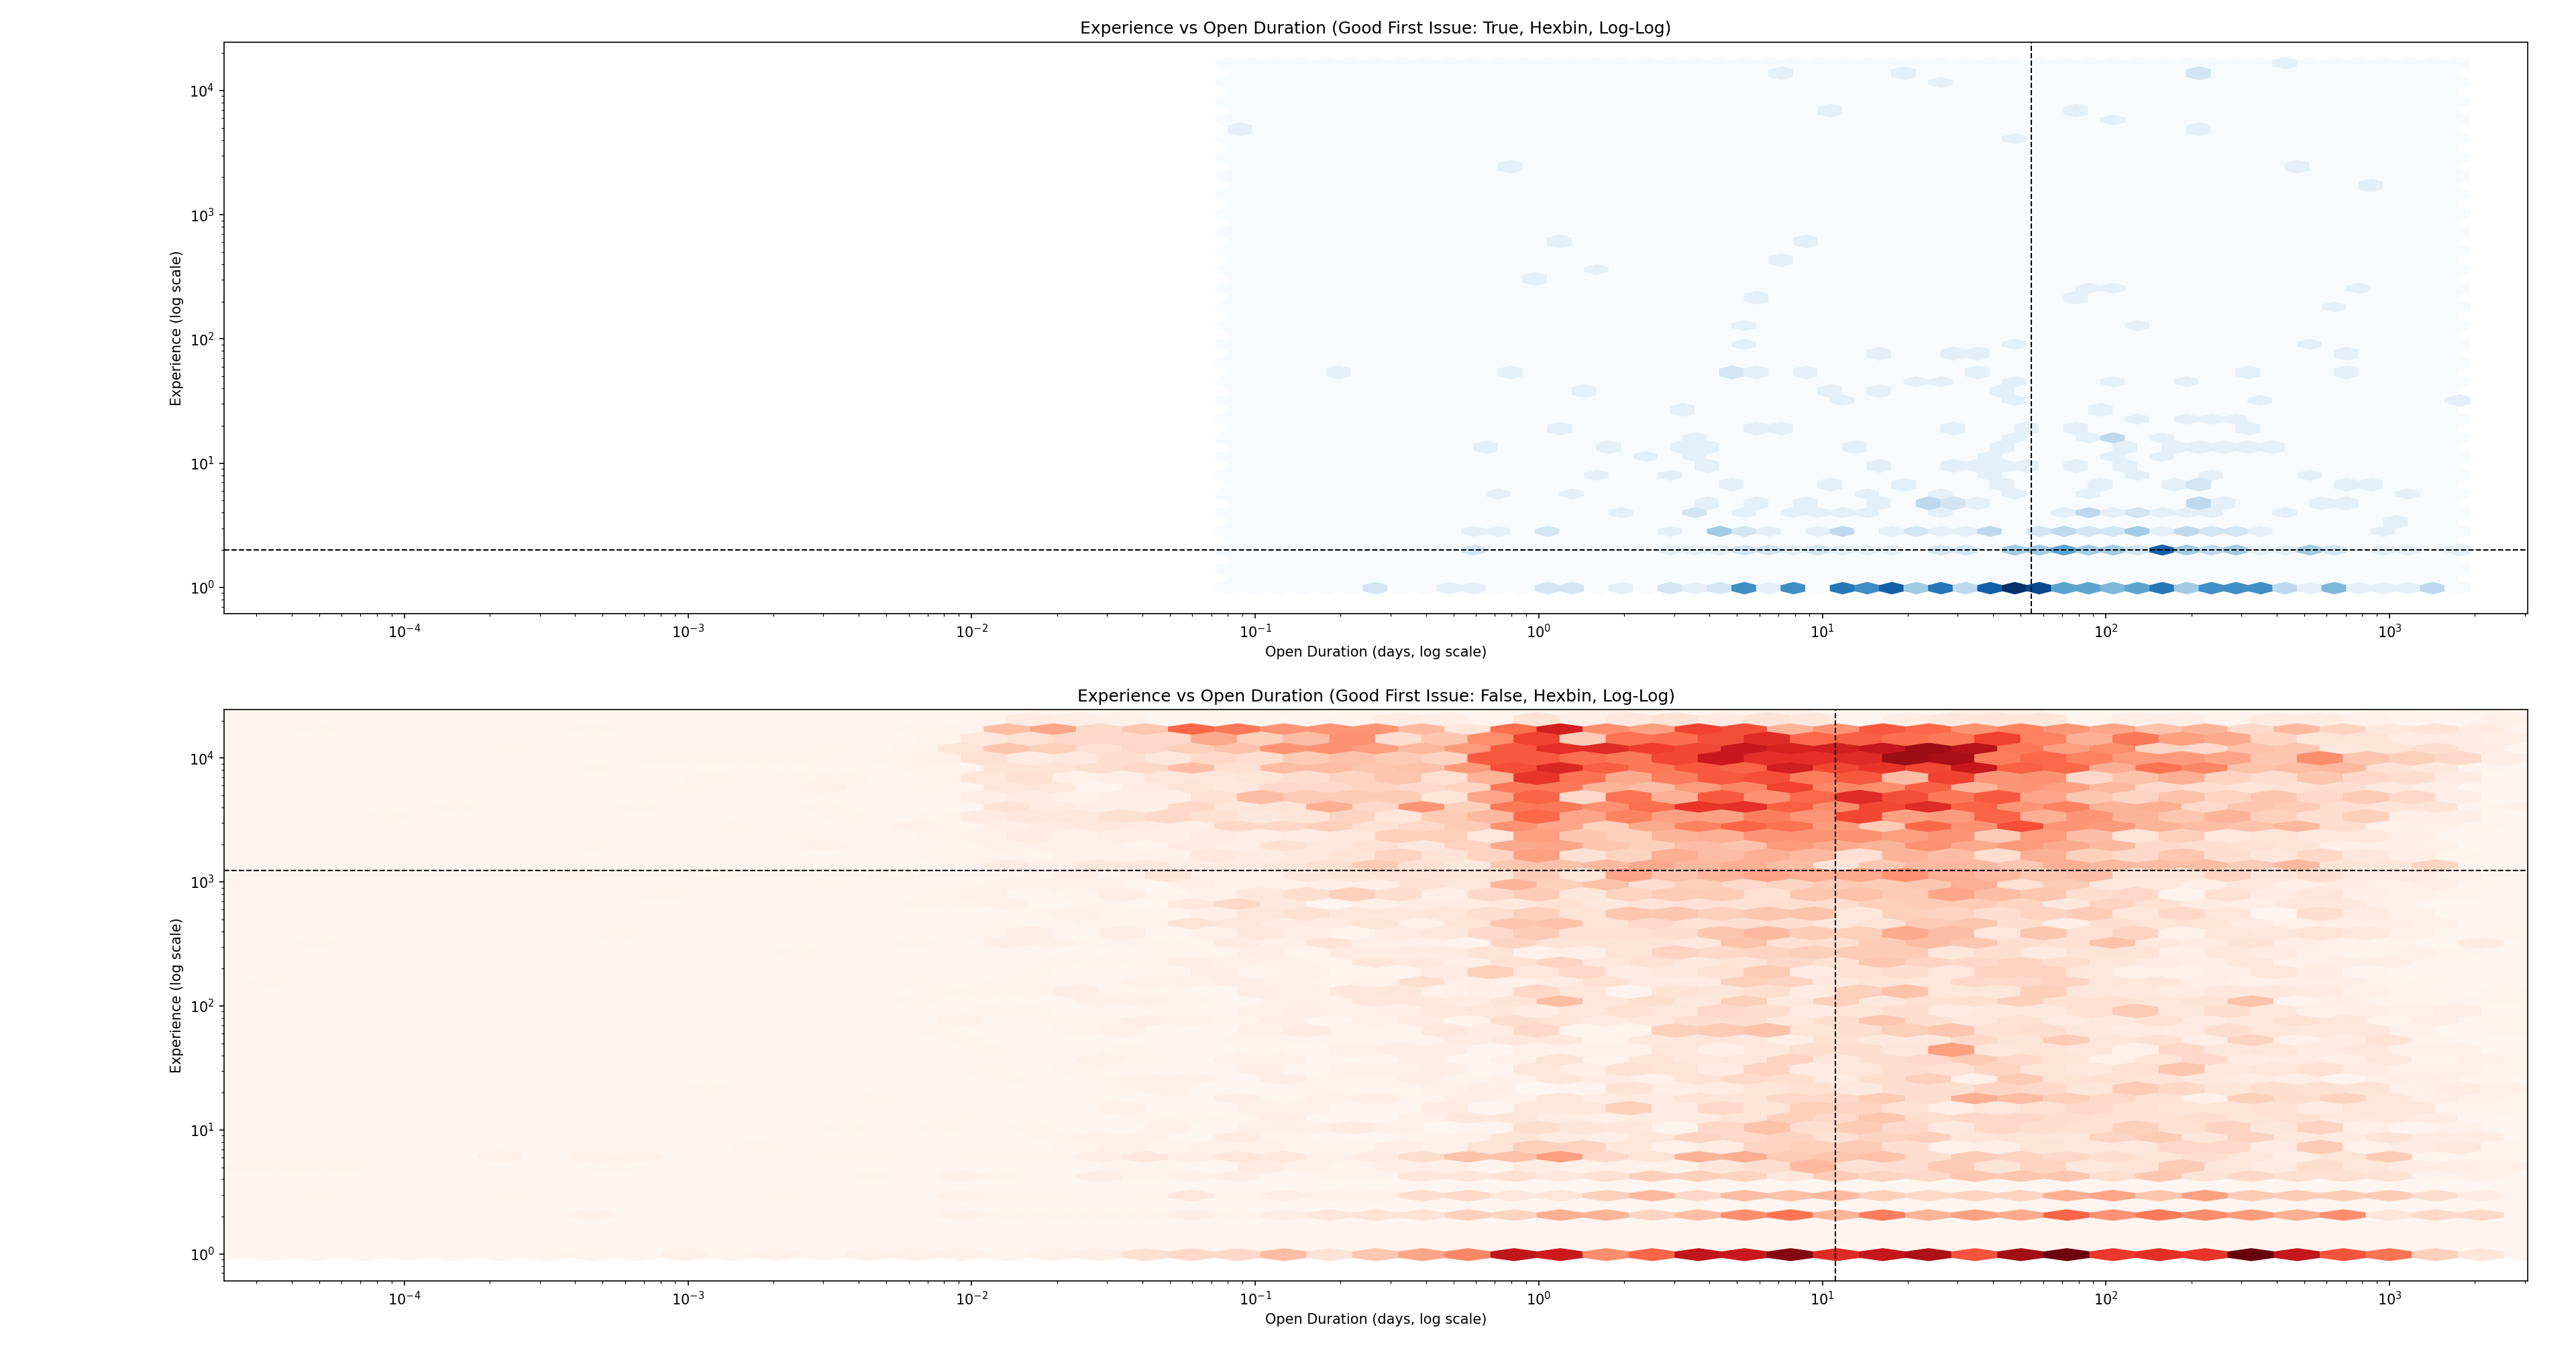
\includegraphics[width=0.9\linewidth]{@BSthesis2024_Nakai/BSthesis2024_Nakai_fig/hexbin.png}}
\caption{RQ2結果}
\label{fig:milestone}
\end{figure*}
%-------------------

\section{RQ3: \RQThree}

\subsection{概要}

ゲーム理論を用いて熟練者にとって最も合理的なふるまいは何かを分析する 

\subsection{手法}

\subsection{結果}

\chapter{考察}

\section{結果の考察}

\subsection{RQ1:Good First Issue に貢献している開発者のうち,新参開発者の割合はどの程度か }
図\todo{番号}の箱ひげ図をもとに,考察する.GFI解決者の経験値の中央値は2であったことから,先行研究\cite{GFI_half}での指摘の通り,半数以上のGFIが初めての貢献でないことが言える.GFIを解決した人の経験値は通常Issueを解決した人の経験値より全体的に低かった.このことから,GFIは``First Issue"とはいえなくても,経験の浅い開発者によって解決されているため新参者向けのIssueとして十分な役割を果たしているといえる.

多くのGFIが新参者によって解決されてはいるが,経験値が10を超えるような新参者とは言い難い開発者がGFIを解決するケースも見られた.特に,通常Issueの経験値の中央値である1237.5を超える開発者がGFIを解決するケースも見られた.これは,プロジェクトの中でも比較的経験豊富な開発者がGFIを解決する場合があることを示している.熟練者がGFIを解決するケースについて,以下のような原因が考えられる.

\def\labelenumi{(\theenumi)}

\begin{enumerate}
  \item GFIを早急に解決する必要性があり,新参者が現れるのを熟練者は待てなかった
  \item あまりにも長期間GFIに貢献する新参者が現れなかったため,熟練者が代わりに解決した
  \item GFIラベルが付いてはいたものの,GFIとして適切なIssue内容ではなかったがラベルの修正が行われなかった
\end{enumerate}

(1),(2)の原因についてはいずれも新参者が現れるまでの時間が関係している.そこで,RQ2ではIssueが開放されている時間と解決者の経験値の関係について考察する.

\subsection{RQ2:熟練者は新参開発者をどの程度待っているか}

図\todo{番号}の箱ひげ図をもとに,GFIの開放期間について考察する.開放期間の最大値は3067.111770833333日であった.これは,Issueが立てられてからCLOSEされるまでに8年以上の期間を要したことを示している.このようなケースでは長期間かけてIssueが解決されているとは考えづらく,解決済みのIssueをCLOSE状態にするのを忘れていたなど他の理由が考えられる.開放期間の頻度を正規化したヒストグラムを図\todo{番号}に示す.

%-------------------
\begin{figure*}[t]
\centerline{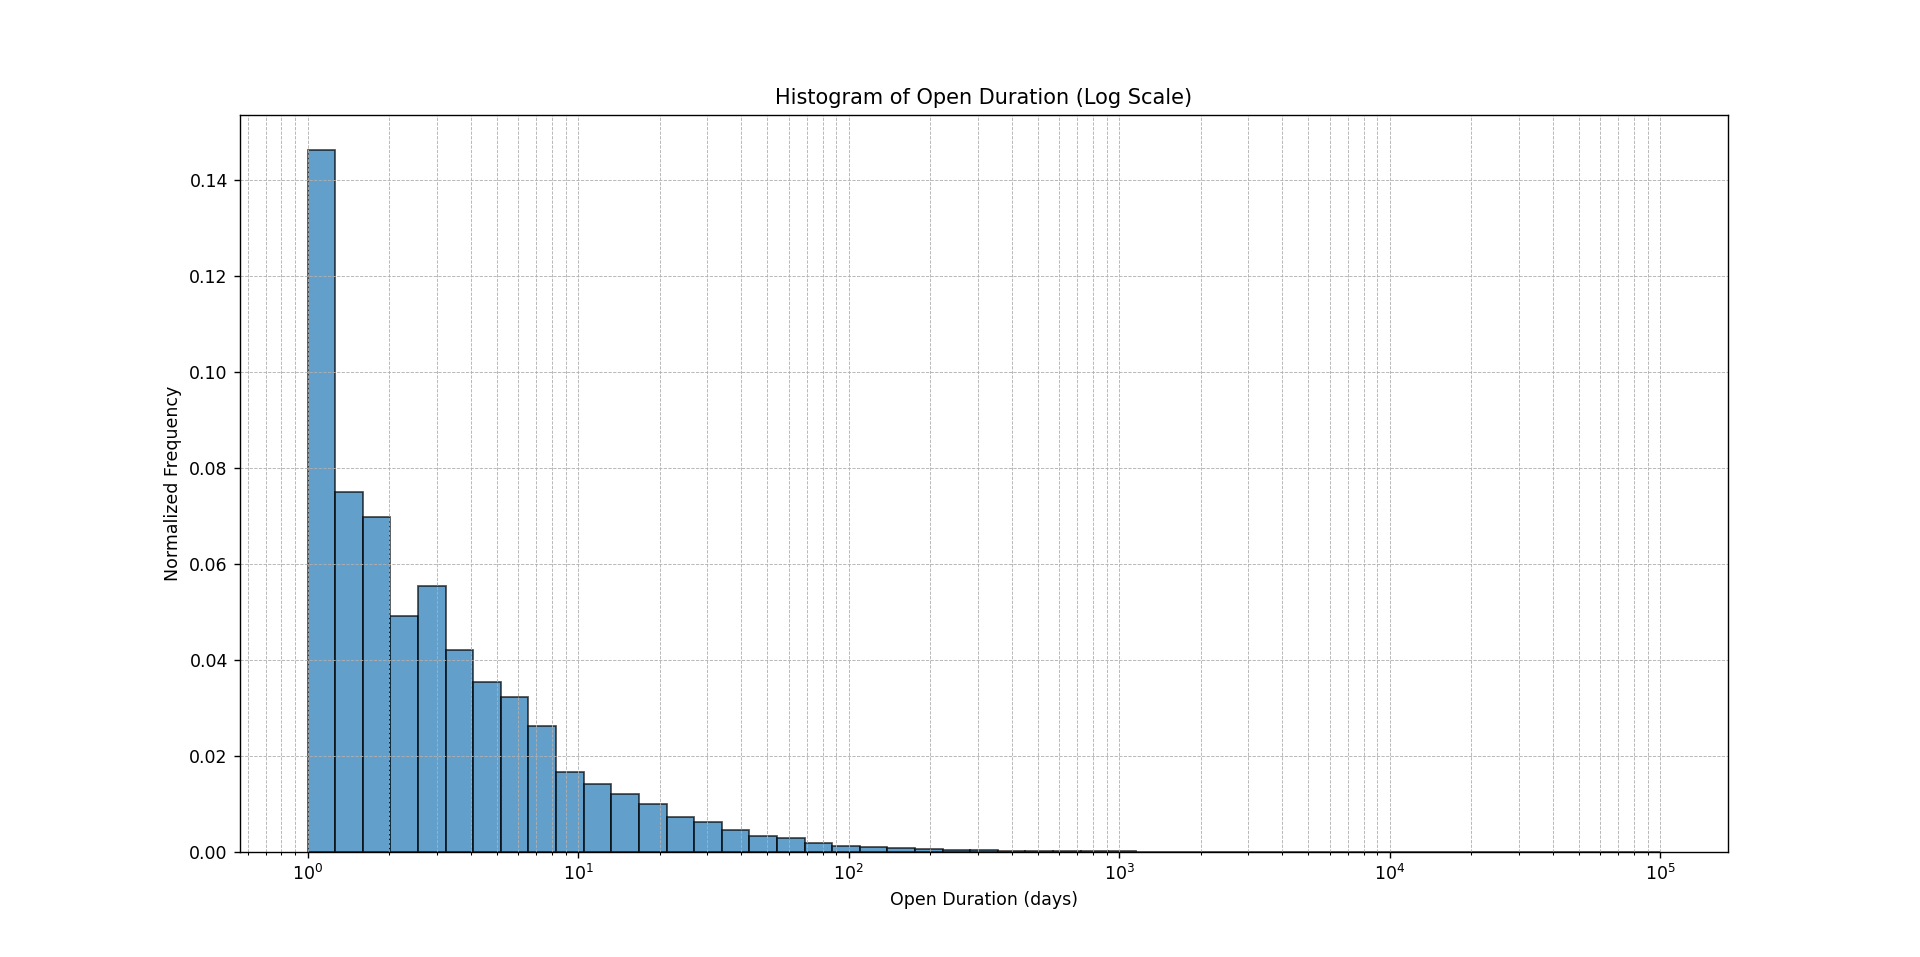
\includegraphics[width=0.9\linewidth]{@BSthesis2024_Nakai/BSthesis2024_Nakai_fig/time_hist.png}}
\caption{開放期間のヒストグラム}
\label{fig:milestone}
\end{figure*}
%-------------------

図\todo{番号}から,開放期間が1000日を超えるようなIssueはほとんど出現しないことがわかる.そこで,開放期間が1000日を超えるIssueを外れ値として扱い,該当する5725件を除外した結果を図\todo{番号}に示す.

%-------------------
\begin{figure*}[t]
\centerline{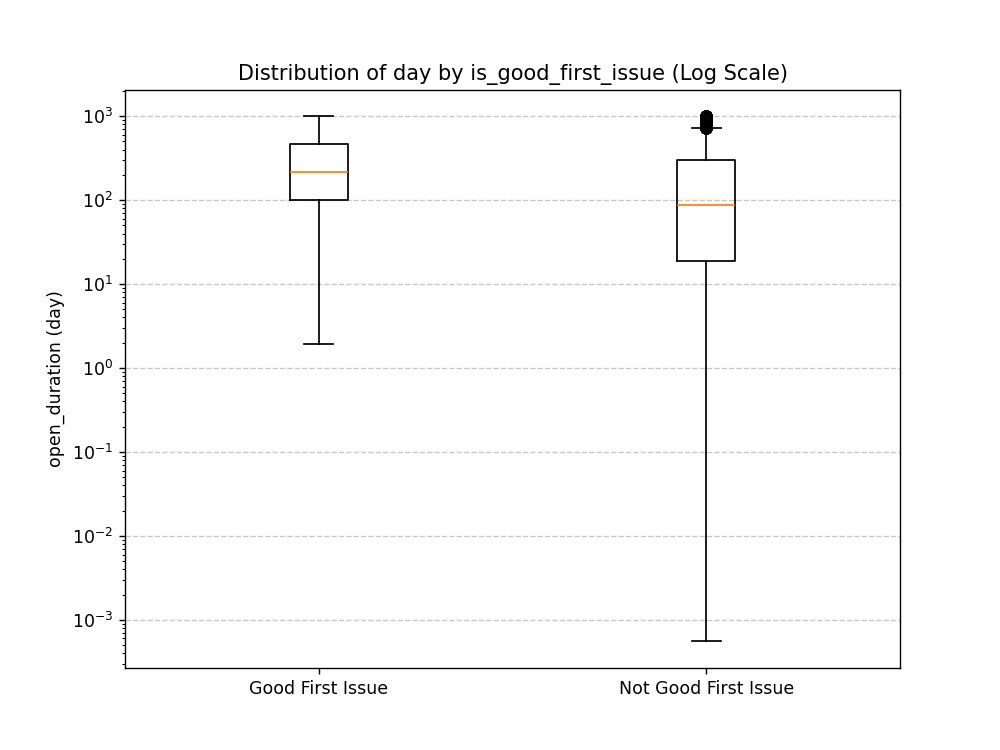
\includegraphics[width=0.9\linewidth]{@BSthesis2024_Nakai/BSthesis2024_Nakai_fig/true_time_box.png}}
\caption{開放期間の箱ひげ図(外れ値を除外)}
\label{fig:milestone}
\end{figure*}
%-------------------

GFIと通常Issueに有意差はないと帰無仮説を立てたとき,マンホイットニーのU検定を行うとp値は0.00000であった.また,効果量は0.331であった.このことから,外れ値を除外しても2つの分布に有意な差があるといえる.

開放期間について,全体的にGFIは通常Issueに比べて長いことから,GFIは解決までに長い期間を要することが分かる.ただ,通常Issueは開放期間が短い部分の幅が広く,早期に解決される通常Issueが多く存在することを示している.GFIは解決が容易なIssueが割り当てられることが多いが,修正に必要な工程が少なく早期解決が見込まれるようなIssueには割り当てられることが少ない.このようなIssueは新参貢献者の研鑽を積むことには不適であるとプロジェクトは判断しているからである.

\subsection{RQ3:熟練者はなぜゲーム理論に基づく合理的なふるまいをしないのか }

\section{妥当性への脅威}

\subsection{内的妥当性}

\subsection{外的妥当性}

\chapter{おわりに}



%%
%% 謝辞
%%
\begin{acknowledgements}
感謝します.
\end{acknowledgements}

%%
%% 参考文献
%%
\begin{thebibliography}{99}

\bibitem{definding}
    Kevin Crowston, Hala Annabi, and James Howison. Defining Open Source Software Project
Success. In In Proceedings of 24th the International Conference on Information Systems
(ICIS 2003), pp. 327–340, 2003

\bibitem{choice}
    Igor Steinmacher, Tayana Conte, and Marco Aurelio Gerosa. Understanding and Supporting
the Choice of an Appropriate Task to Start with in Open Source Software Communities.
In In Proceedings of the 48th Hawaii International Conference on System Sciences (HICSS
2015), pp. 5299–5308, 2015.

\bibitem{GFI}
    堀口 日向. OSSプロジェクトへのオンボーディング支援のためのGood First Issue自動分類 2022.

\bibitem{OTC}
    Amanda Lee, Jeffrey C. Carver, and Amiangshu Bosu. Understanding the Impressions,
Motivations, and Barriers of One Time Code Contributors to FLOSS Projects: A Survey.
In Proceedings of the 39th International Conference on Software Engineering (ICSE 2017),
pp. 187–197, 2017.

\bibitem{sosial}
C. Casalnuovo, B. Vasilescu, P. Devanbu, and V. Filkov, “Developer
onboarding in GitHub: The role of prior social links and language experience,” in Proc. Joint Meeting on Foundations of Software Engineering
(ESEC/FSE), 2015, p. 817–828.

\bibitem{menter1}
Fabian Fagerholm, Alejandro Guinea, Jay Borenstein, and J¨urgen M¨unch. Onboarding in
Open Source Projects. IEEE Software, Vol. 31, No. 6, pp. 54–61, 2014.

\bibitem{menter2}
 Ricardo Britto, Darja Smite, Lars-Ola Damm, and J¨urgen B¨orstler. Performance Evolution
of Newcomers in Large-Scale Distributed Software Projects: An Industrial Case Study. In In
Proceedings of the 14th International Conference on Global Software Engineering (ICGSE
2019), pp. 1–11, 2019.

\bibitem{portal}
 Igor Steinmacher, Tayana Uchoa Conte, Christoph Treude, and Marco Aur´elio Gerosa.
Overcoming Open Source Project Entry Barriers with a Portal for Newcomers. In In
Proceedings of the 38th International Conference on Software Engineering (ICSE 2016),
pp. 273–284, 2016.

\bibitem{social barries}
Igor Steinmacher, Tayana Conte, Marco Aur´elio Gerosa, and David Redmiles. Social Barriers Faced by Newcomers Placing Their First Contribution in Open Source Software Projects.
In In Proceedings of the 18th ACM Conference on Computer Supported Cooperative Work & Social Computing (CSCW 2015), pp. 1379–1392, 2015.

\bibitem{GFI_half}
Xin Tan, Minghui Zhou, and Zeyu Sun. A First Look at Good First Issues on GitHub. In In
Proceedings of the 28th ACM Joint Meeting on European Software Engineering Conference
and Symposium on the Foundations of Software Engineering (ESEC/FSE 2020), pp. 398–
409, 2020.

\bibitem{game_theory}
岡田 章,ゲーム理論 (新版)),株式会社有斐閣,2011 年. 

\bibitem{}

\end{thebibliography}

%%%%%%%%%%%%%%%%%%%%%%%%%%%%%%%%%%%%%%%%%%%%%%%%%%%%%%%%%%%%%%%%%%%%%%%%

%%
%% 付録
%%
% \appendix
% 
% \chapter{サンプルプログラム}
% 
% プログラムリストや実行結果など,本論を補足する上で必要と思われるものが
% あれば付録として付ける.
% 
% {
% \footnotesize
% \begin{verbatim}
% #include <stdio.h>
% int main(void)
% {
%     printf("Hello, World!\n");
%     return 0;
% }
% \end{verbatim}
% }

%%%%%%%%%%%%%%%%%%%%%%%%%%%%%%%%%%%%%%%%%%%%%%%%%%%%%%%%%%%%%%%%%%%%%%%%

\end{document}
